%!TEX root = ../main.tex

\section*{Ejercicio 6}
El operador Laplaciano en 2D se define como:

$$
\nabla^2 u(x, y)=\frac{\partial^2 u}{\partial x^2}+\frac{\partial^2 u}{\partial y^2}
$$

donde $u(x, y)$ es una función que representa la intensidad de los pixeles de la imagen en el dominio espacial. El operador Laplaciano se utiliza para detectar bordes porque responde a las variaciones de la intensidad de los pixeles en la vecindad de cada punto. En áreas de la imagen donde la intensidad varía rápidamente (bordes), el Laplaciano tiene un valor alto, mientras que en áreas homogéneas (sin bordes) el Laplaciano es cercano a cero. El proceso de detección de bordes implica calcular el Laplaciano de la imagen $u(x, y)$, lo que da como resultado un mapa de bordes.

En este ejercicio estamos interesados en reconstruir la imagen original $u(x, y)$ a partir de los bordes detectados. Para esto debemos resolver la ecuación de Poisson en 2D

$$
\nabla^2 u(x, y)=f(x, y)
$$

donde $f(x, y)$ es el mapa de bordes.
El problema (1) puede ser discretizado en un sistema de ecuaciones lineales de la forma:

$$
A u=f
$$

donde $A$ es una matriz que representa el operador Laplaciano discreto, $u$ es el vector que contiene los valores de la imagen original en cada pixel (a reconstruir), y $f$ es el vector que contiene los valores de los bordes detectados.\\

\textbf{Solución.} Lo primero que debemos hacer es  discretizar el laplaciano,  para esto usamos el teorema de Taylor. A saber

    $$u(x+h,y)=u(x,y)+h u_x(x,y)+\frac{h^2\partial^2_{x}u(x,y)}{2}+O(h^3),$$
    $$u(x-h,y)=u(x,y)-h u_x(x,y)+\frac{h^2\partial^2_x u(x,y)}{2}+O(h^3),$$

    realizando esto para $u(x,y+h)$ y $u(x,y-h)$ obtenemos que

    $$\Delta u(x, y) \approx \frac{u(x-h, y)+u(x+h, y)+u(x, y-h)+u(x, y+h)-4 u(x, y)}{h^2}.$$

    Para reconstruir la imágen debemos encontrar $u(x,y)$, la función que nos da la intensidad de cada pixel, esto es resolver la ecuación de  Poisson $\Delta u(x,y)= f(x,y)$ donde $f(x,y)$ es el mapa de bordes. Primero consideremos para el problema una malla regular, tomaremos $h=1$ ya que cada pixel representa un paso, en una  dimensión la matriz que obtenemos es tridiagonal, sin embargo al discretizar la ecuación de Poisson en 2D debemos mover $f$ en coordenadas $x$ y $y$, por lo tanto debemos analizarlo con detalle.\\

    Como usamos usa malla regular de $n \times n$ (porque el problema es  2D), cada fila de la matriz sería de $n\times n$, obteniendo

    \[
    \Delta u_{ij} =  u_{i+1, j} + u_{i-1, j} + u_{i, j+1} + u_{i, j-1} - 4 u_{ij} = f_{ij}
    \]

    donde \(2 \leq i \leq m-1\) y \(2 \leq j \leq n-1\). Esto da lugar a un sistema lineal de dimensión \(n^2 \times  n^2\),  $A u=f$, donde 

    $$
    A=\left[\begin{array}{ccccccc}
    D & I & 0 & 0 & 0 & \cdots & 0 \\
    I & D & I & 0 & 0 & \cdots & 0 \\
    0 & I & D & I & 0 & \cdots & 0 \\
    \vdots & \ddots & \ddots & \ddots & \ddots & \ddots & \vdots \\
    0 & \cdots & 0 & I & D & I & 0 \\
    0 & \cdots & \cdots & 0 & I & D & I \\
    0 & \cdots & \cdots & \cdots & 0 & I & D
    \end{array}\right], \text{ donde }  D=\left[\begin{array}{ccccccc}
    -4 & 1 & 0 & 0 & 0 & \cdots & 0 \\
    1 & -4 & 1 & 0 & 0 & \cdots & 0 \\
    0 & 1 & -4 & 1 & 0 & \cdots & 0 \\
    \vdots & \ddots & \ddots & \ddots & \ddots & \ddots & \vdots \\
    0 & \cdots & 0 & 1 & -4 & 1 & 0 \\
    0 & \cdots & \cdots & 0 & 1 & -4 & 1 \\
    0 & \cdots & \cdots & \cdots & 0 & 1 & -4
    \end{array}\right],
    $$

    y como $f$ es una matriz, se debe aplanar como vector columna. Por ejemplo en $3\times 3$

    $$
    A=\left[\begin{array}{ccc|ccc|ccc}
    -4 & 1 & 0 & 1 & 0 & 0 & 0 & 0 & 0 \\
    1 & -4 & 1 & 0 & 1 & 0 & 0 & 0 & 0 \\
    0 & 1 & -4 & 0 & 0 & 1 & 0 & 0 & 0 \\
    \hline1 & 0 & 0 & -4 & 1 & 0 & 1 & 0 & 0 \\
    0 & 1 & 0 & 1 & -4 & 1 & 0 & 1 & 0 \\
    0 & 0 & 1 & 0 & 1 & -4 & 0 & 0 & 1 \\
    \hline 0 & 0 & 0 & 1 & 0 & 0 & -4 & 1 & 0 \\
    0 & 0 & 0 & 0 & 1 & 0 & 1 & -4 & 1 \\
    0 & 0 & 0 & 0 & 0 & 1 & 0 & 1 & -4
    \end{array}\right].
    $$

    Ahora debemos resolver los sistemas implementando los métodos de Jacobi,Gauss-Seidel y SOR, esto lo hicimos en Matlab y el código es extenso, por lo que lo adjuntamos en el cuaderno de Jupyter, sin embargo vamos a ver aquí los resultados obtenidos.\\

    Para el método de Jacobi aprovechamos que la inversa de la matriz diagonal es simplemente invertir la diagonal, a saber $1/a_{ii}$, luego el código es bastante eficiente y puede correr 100 iteraciones muy rápido. \\

    En Gauss-Seidel no fue posible implementar el método de manera  matricial, invertir matriz $(D-L)$ es un trabajo costoso teniendo en cuenta que la primera imagen es de $240\times 240$, es decir una matriz de $57600\times 57600$, una sola iteración costaba varios minutos. En vista de esto optamos por implementar el método resolviendo cada ecuación y sin definir la matriz $A$, usando claramente que 

     \[
    \Delta u_{ij} =  u_{i+1, j} + u_{i-1, j} + u_{i, j+1} + u_{i, j-1} - 4 u_{ij} = f_{ij},
    \]

    se obtiene una  fórmula eficiente para hace Gauss-Seidel, a saber

    $$u_{i j}^{(k+1)}=\frac{1}{4}\left(\left(u_{i+1, j}^{(k)}+u_{i-1, j}^{(k+1)}+u_{i, j+1}^{(k)}+u_{i, j-1}^{(k+1)}\right)-f_{i j}\right),$$

    esto nos permitió implementar todo de manera  eficiente. Para SOR la idea fue exactamente la misma pero aplicando la relajación 

    $$u_{ij}^{k+1}=(1-\omega )u_{ij}^{k}+\frac{\omega}{4}\left(\left(u_{i+1, j}^{(k)}+u_{i-1, j}^{(k+1)}+u_{i, j+1}^{(k)}+u_{i, j-1}^{(k+1)}\right)-f_{i j}\right),$$

    en este caso tomamos $\omega=1.5$ ya que la idea era acelerar  la convergencia, esto se logra con $1<\omega<2$. Finalmente para la primera imagen, dada por el archivo Bordes1, obtuvimos los siguientes resultados aplicando 100 iteraciones.

    \begin{center}
        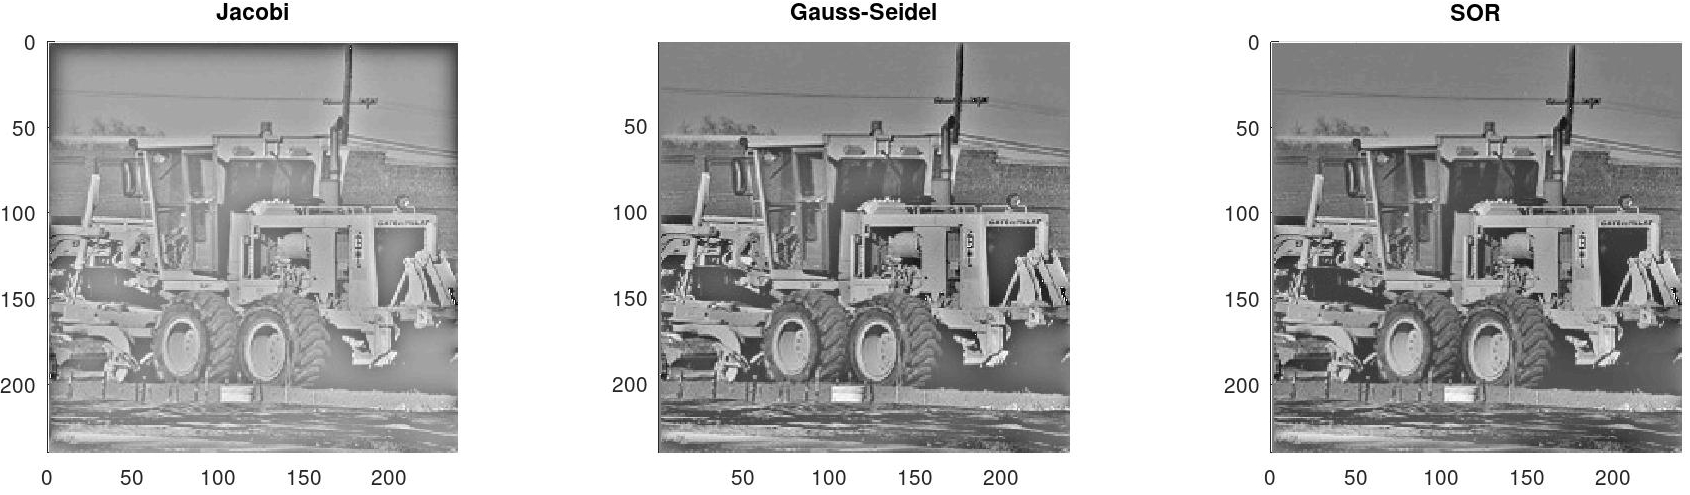
\includegraphics[scale=0.27]{Graficas/Bordes1.jpg}
    \end{center}

    Para la segunda imagen también aplicamos 100 iteraciones, obtuvimos 

    \begin{center}
        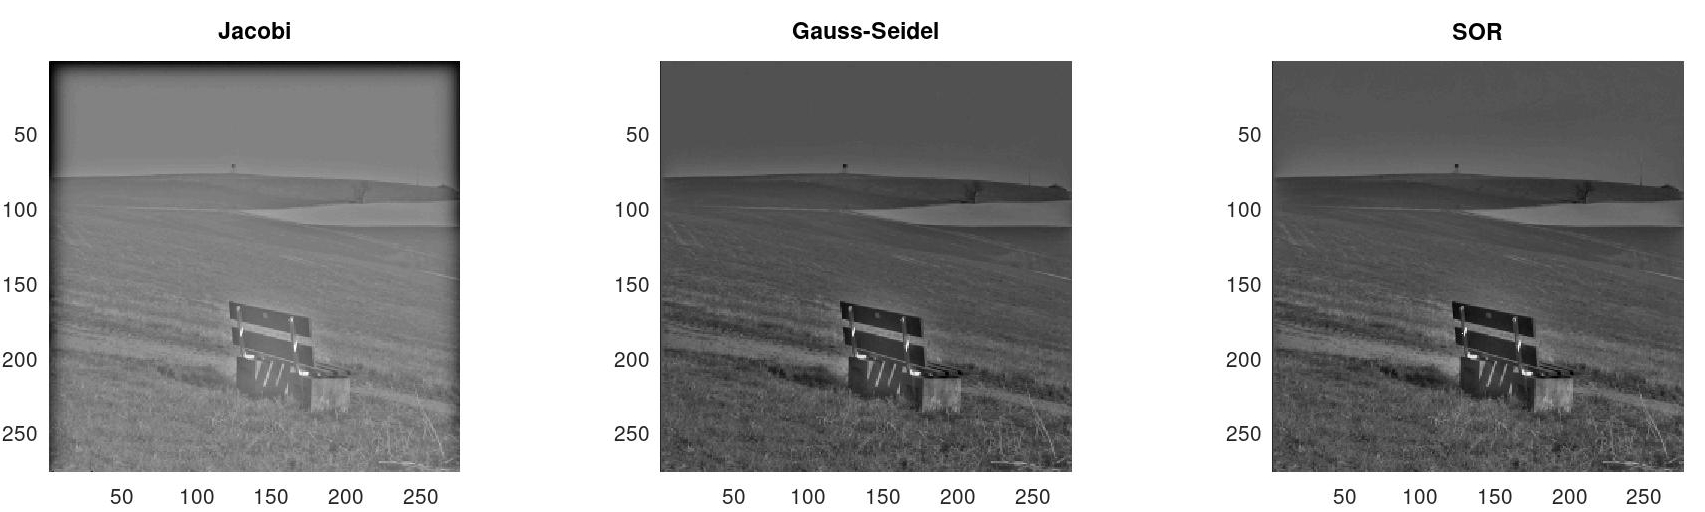
\includegraphics[scale=0.27]{Graficas/Bordes2.jpg}
    \end{center}

    Aplicamos 100 iteraciones para que se observara diferencia entre los métodos ya que con muchas iteraciones el problema se estabiliza de manera que no notaremos diferencia entre aplicar un método y otro.